% exemples d'IR EAD et EAC
% exemples d'image de répertoire


\appendix
\part*{Annexes}
\addcontentsline{toc}{part}{Annexes}
\pagestyle{myheadings}
\markboth{Annexes}{Annexes}

Les annexes présentent à la fois les livrables effectués durant le stage et des compléments au présent mémoire. Cette partie contient également les chemins de localisation des fichiers. Ils sont reproduits sur une \citecode{clé usb} et sur un dépôt Github accessible à l'adresse suivante : \url{https://github.com/Lucaterre/L-TERRIEL_memoireDeStage_M2TNAH_ENC}.

\chapter{Sources et Ecosystème Lectaurep}

localisation : \citecode{/A-Sources\_et\_Ecosystème\_Lectaurep/} contenant :

\section{histoire du projet lectaurep}
localisation : \citecode{/A1-histoire\_projet\_lectaurep/} contenant :
\begin{itemize}
    \item \citecode{demande\_ocr\_Ollion.pdf}
\end{itemize}


\section{Extraits du corpus des répertoires de notaires}
localisation : \citecode{A2-Extraits\_du\_corpus\_des\_répertoires\_de\_notaires/} contenant :
\begin{itemize}
    \item \citecode{exemple\_minute.jpg} ou Figure  \ref{fig:exemple_minute}
    \item \citecode{repertoire\_structure\_tableaux.png} ou Figure  \ref{fig:tableaux_repertoires}
\end{itemize}

\section{Outils généraux utilisés dans Lectaurep}

localisation : \citecode{A3-Outils\_de\_Lectaurep} contenant :
\begin{itemize}
    \item \citecode{Interface\_eScriptorium.png} ou Figure \ref{fig:appli_eScriptorium}
    \item \citecode{sharedocs.png} ou Figure \ref{fig:shareDocs}
    \item \citecode{blog\_lectaurep.png} ou Figure \ref{fig:blog_lectaurep}
\end{itemize}
% inclure les figures ici :

\begin{figure}[h!]
    \centering
    \centerline{\fbox{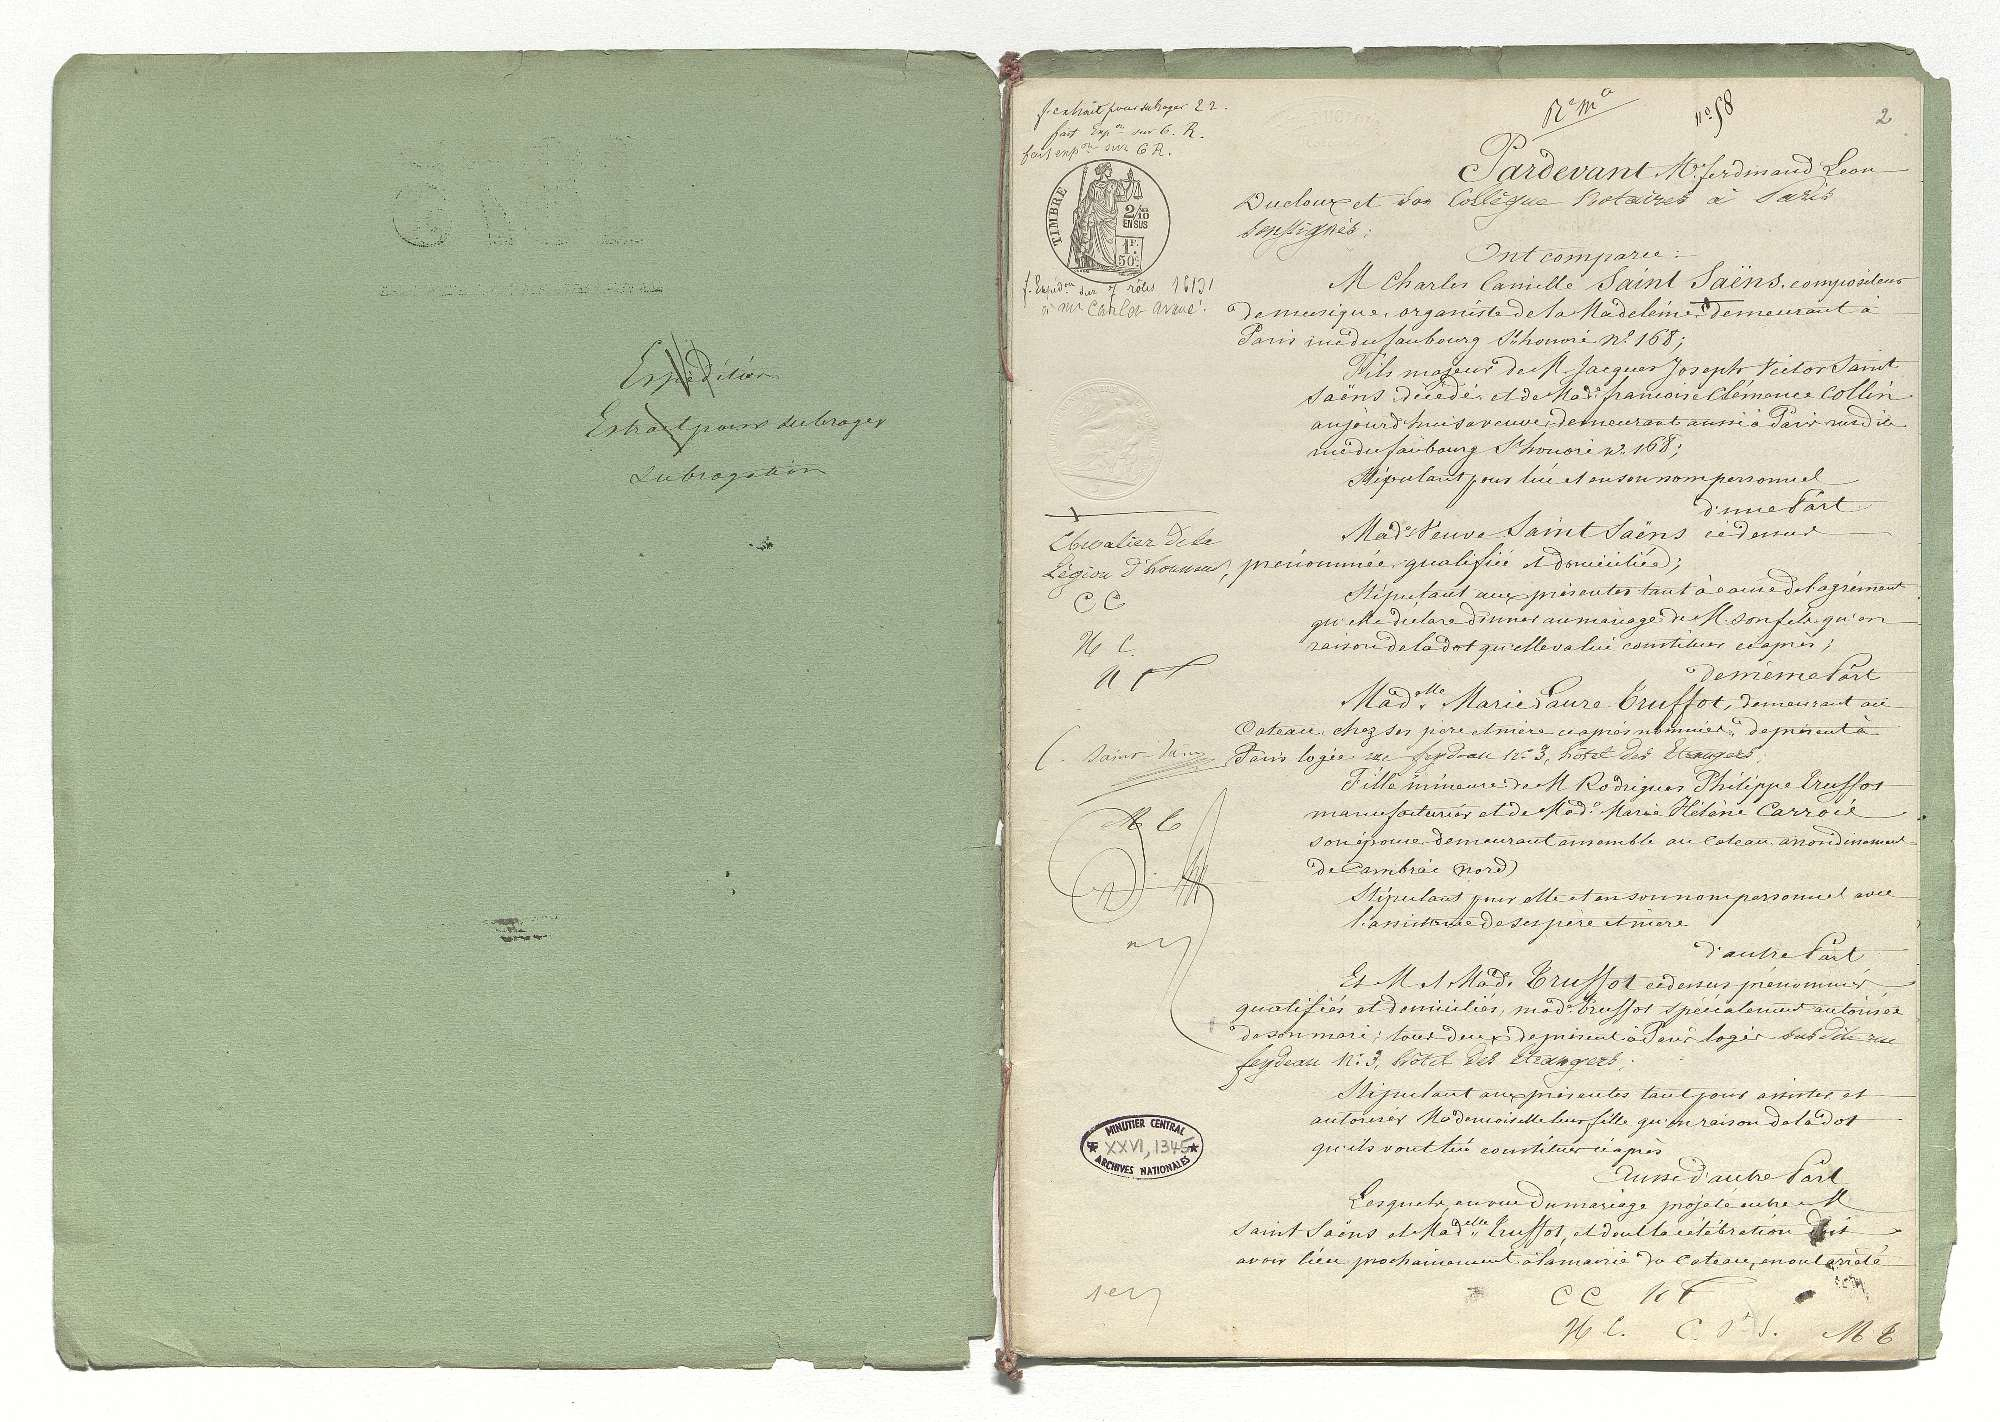
\includegraphics[width=19cm]{images_annexes/exemple_minute.jpg}}}
    \caption{Exemple de minute notariale \textcopyright Archives nationales/DMC, Minute \inquote{Contrat de mariage entre Charles Camille Saint-Saens, compositeur de musique, organiste de la Madeleine demeurant au 168 rue du Faubourg Saint-Honoré, et Marie-Laure Truffot, fille de Rodrigue Truffot, manufacturier au Cateau-Cambrésis}, 18 janvier 1875,  MC/ET/XXVI/1345 (cote originale), MC/RS//872, lien vers la SIV : \url{https://www.siv.archives-nationales.culture.gouv.fr/siv/UD/FRAN_IR_041418/c1p6uqwjl1o3-xlv0cdl5wlgv}(consulté le 14/09/2020).}
    \label{fig:exemple_minute}
\end{figure}

\begin{figure}[h!]
    \centering
    \centerline{\fbox{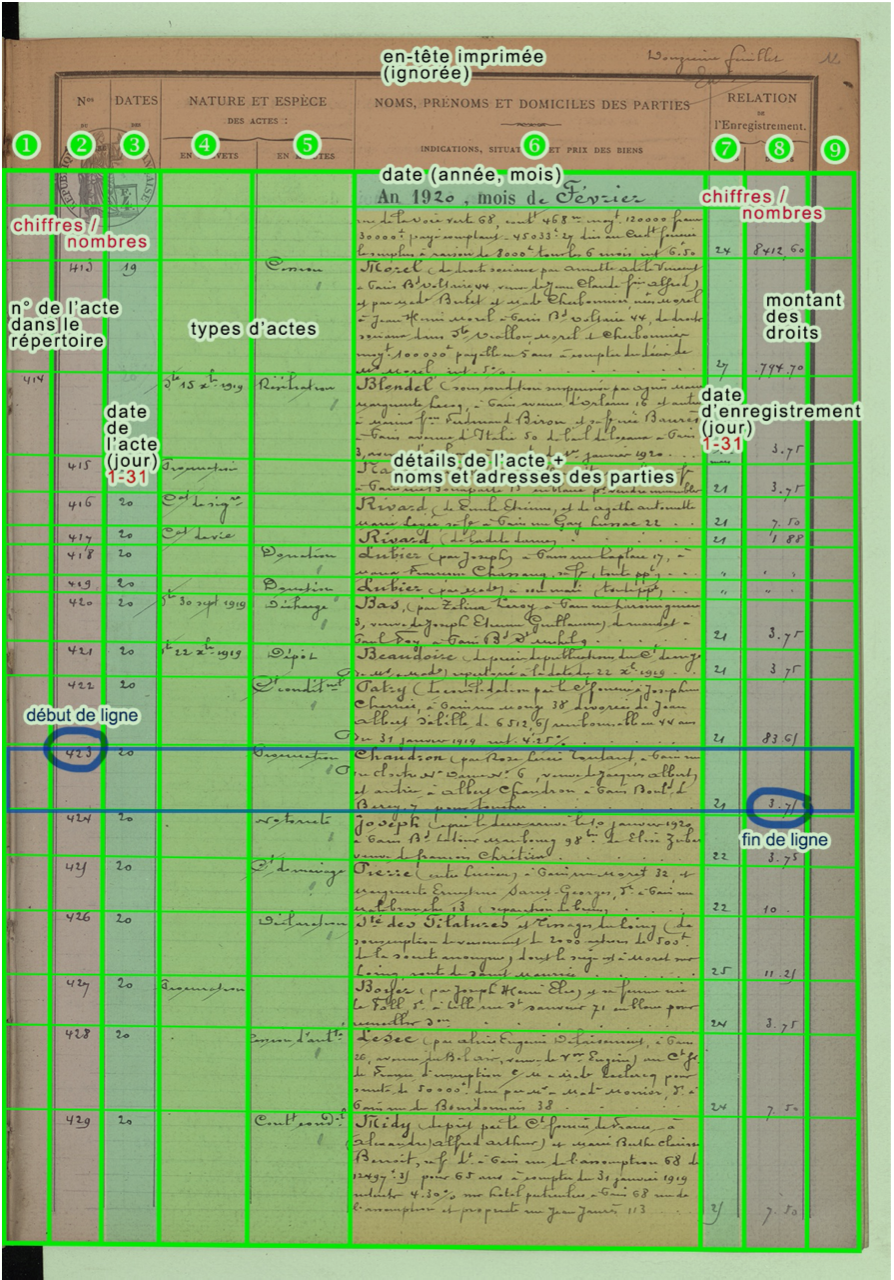
\includegraphics[width=14cm]{images_annexes/repertoire_structure_tableaux.png}}}
    \caption{Structuration en tableaux des répertoires \textcopyright \cite{bonhomme_defis_2018}, pp. 27.} 
    \label{fig:tableaux_repertoires}
\end{figure}

\begin{figure}[h]
    \centering
    \centerline{\fbox{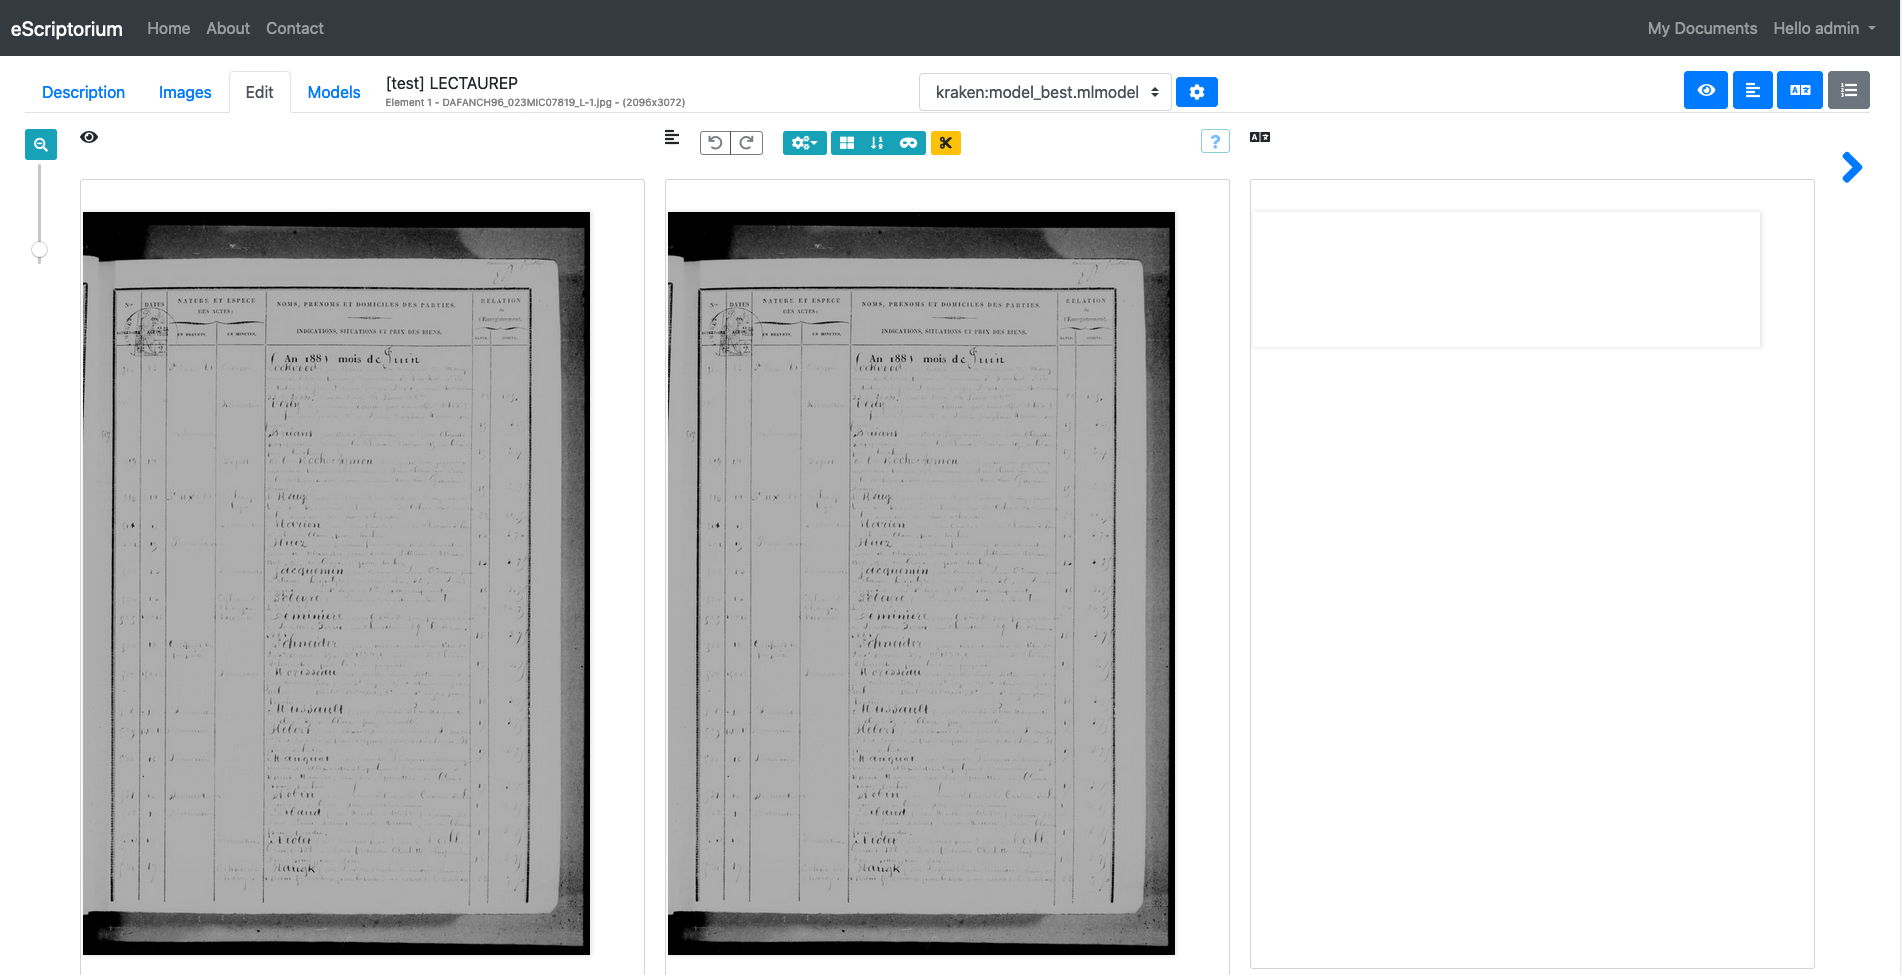
\includegraphics[width=18cm]{images_annexes/interface_eScriptorium.png}}}
    \caption{Application web eScriptorium \textcopyright L. Terriel, 2020, eScriptorium} 
    \label{fig:appli_eScriptorium}
\end{figure}

\begin{figure}[h]
    \centering
    \centerline{\fbox{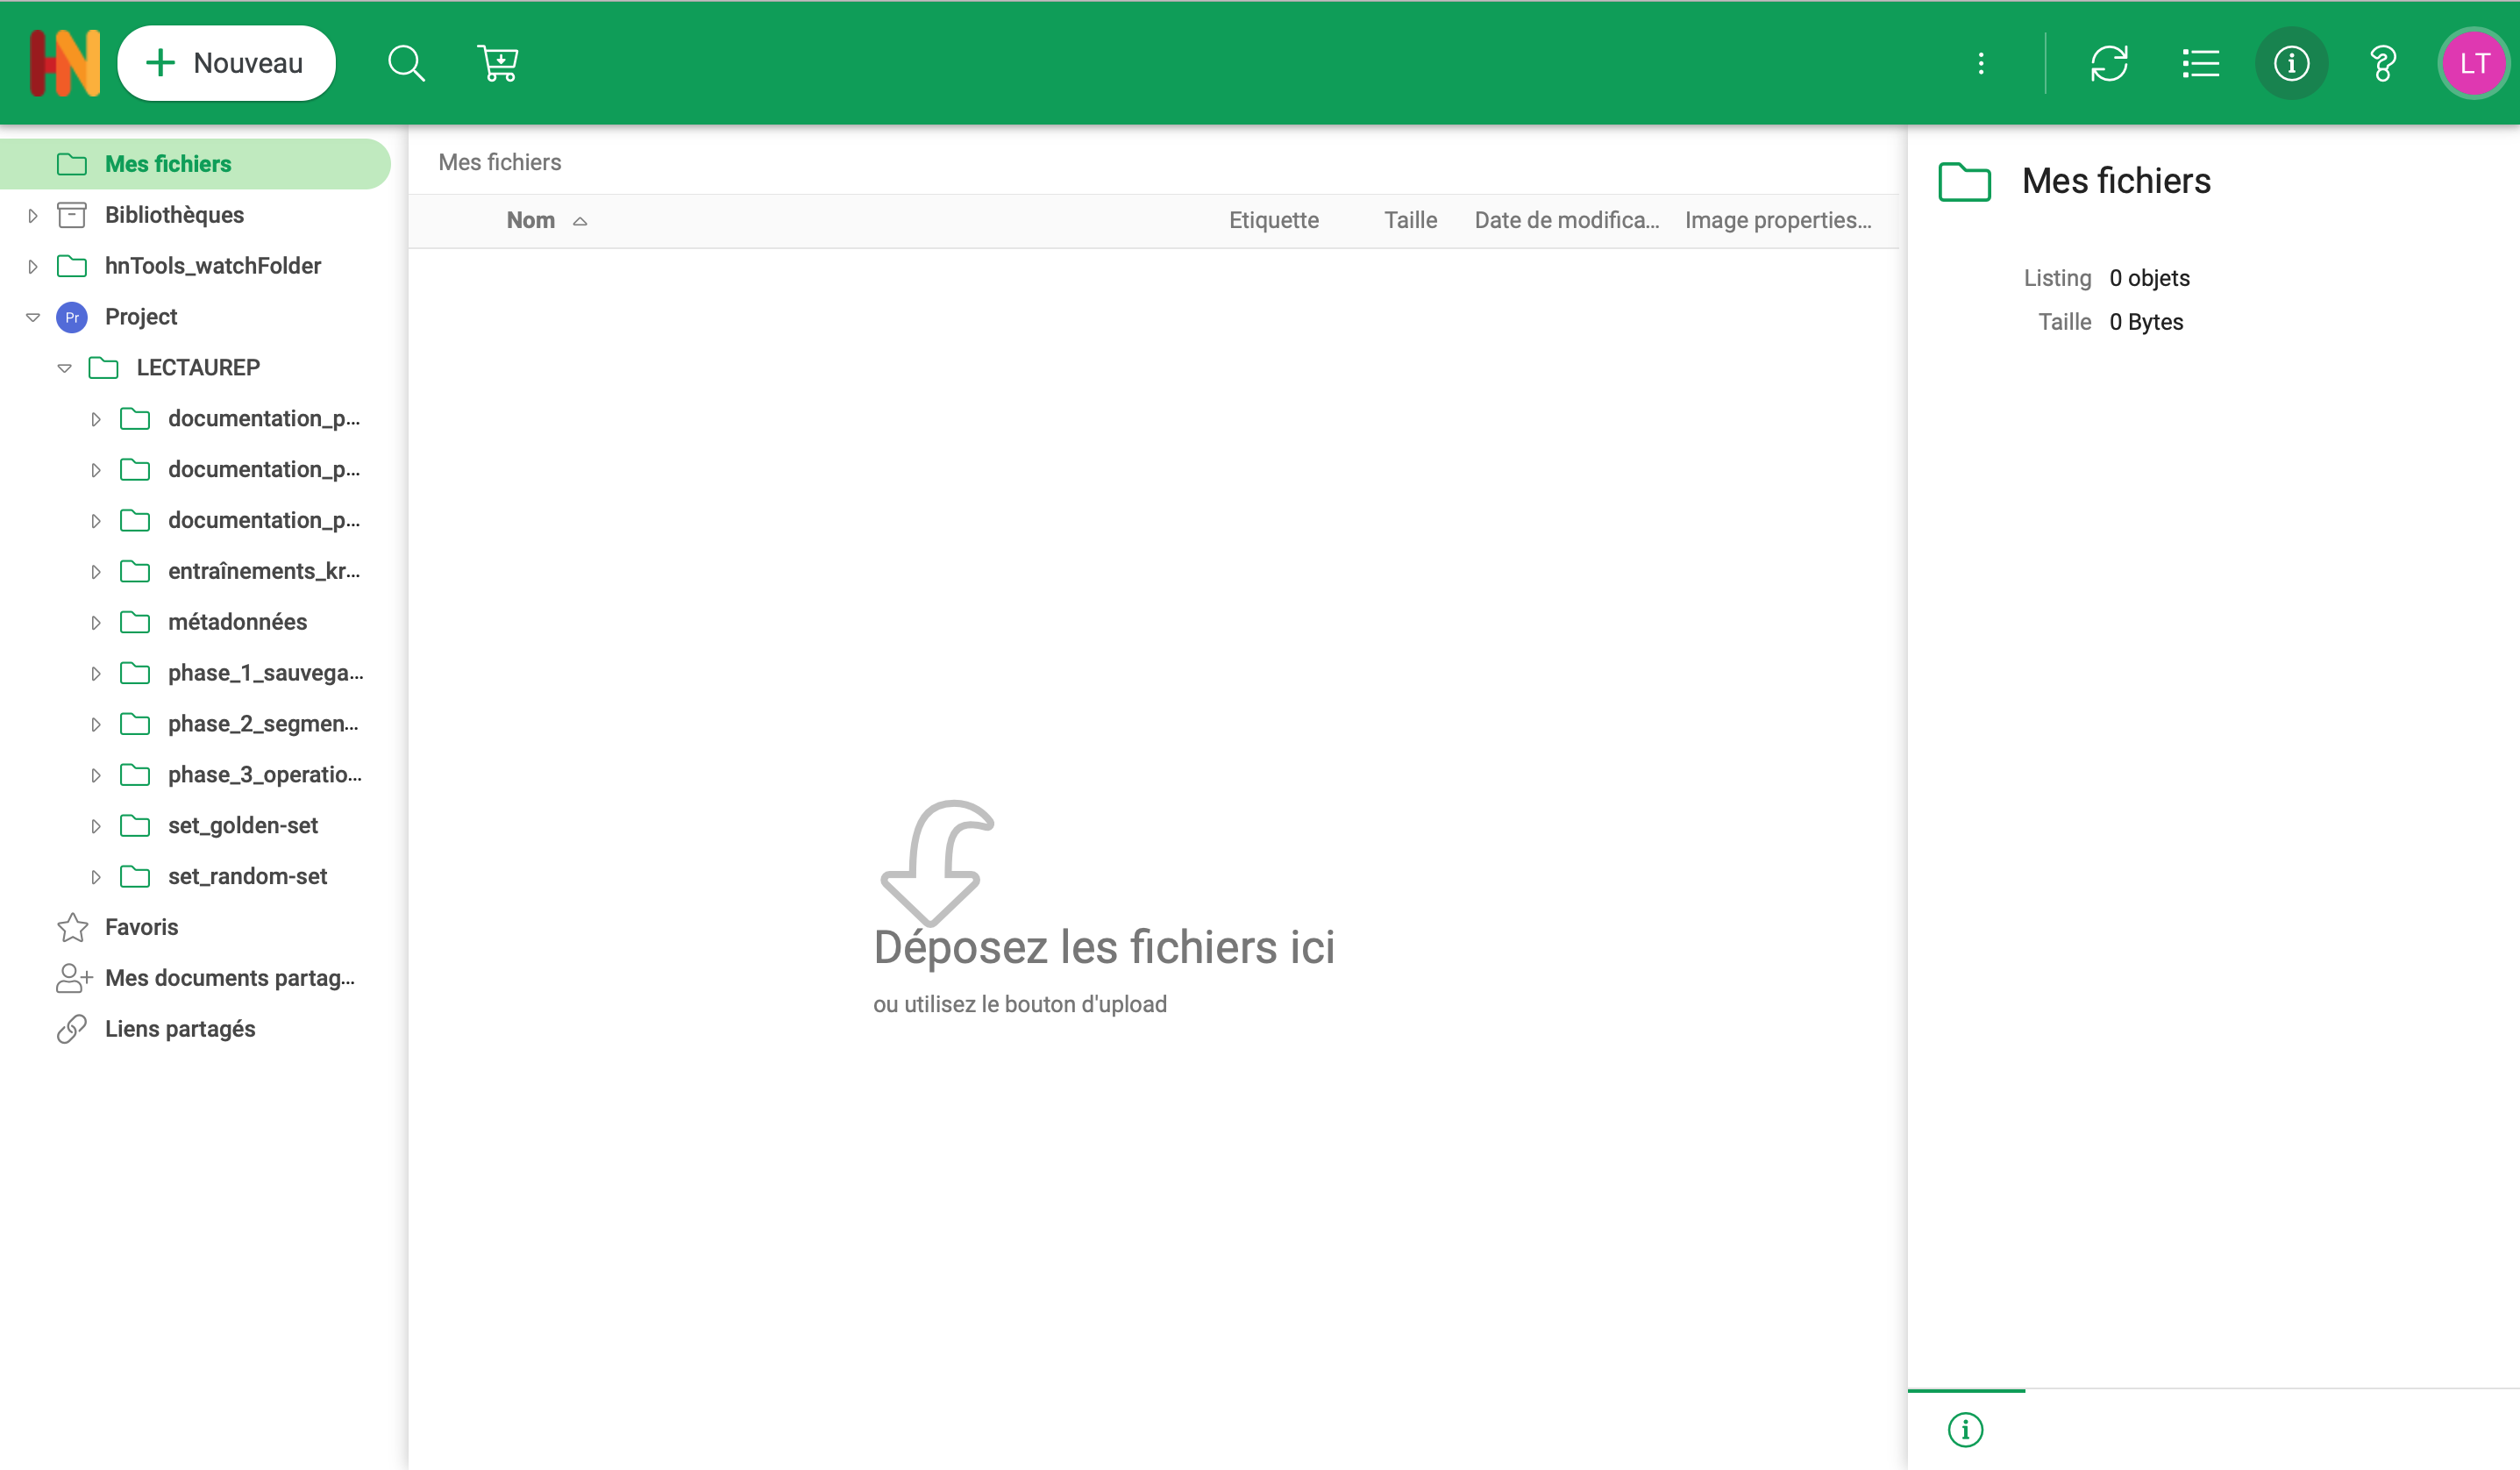
\includegraphics[width=18cm]{images_annexes/sharedocs.png}}}
    \caption{Exemple du \textit{Golden Set} et du \textit{Random Set} stockés sur Sharedocs (Huma-num) \textcopyright L. Terriel, 2020, Sharedocs (Huma-num)} 
    \label{fig:shareDocs}
\end{figure}

\begin{figure}[h]
    \centering
    \centerline{\fbox{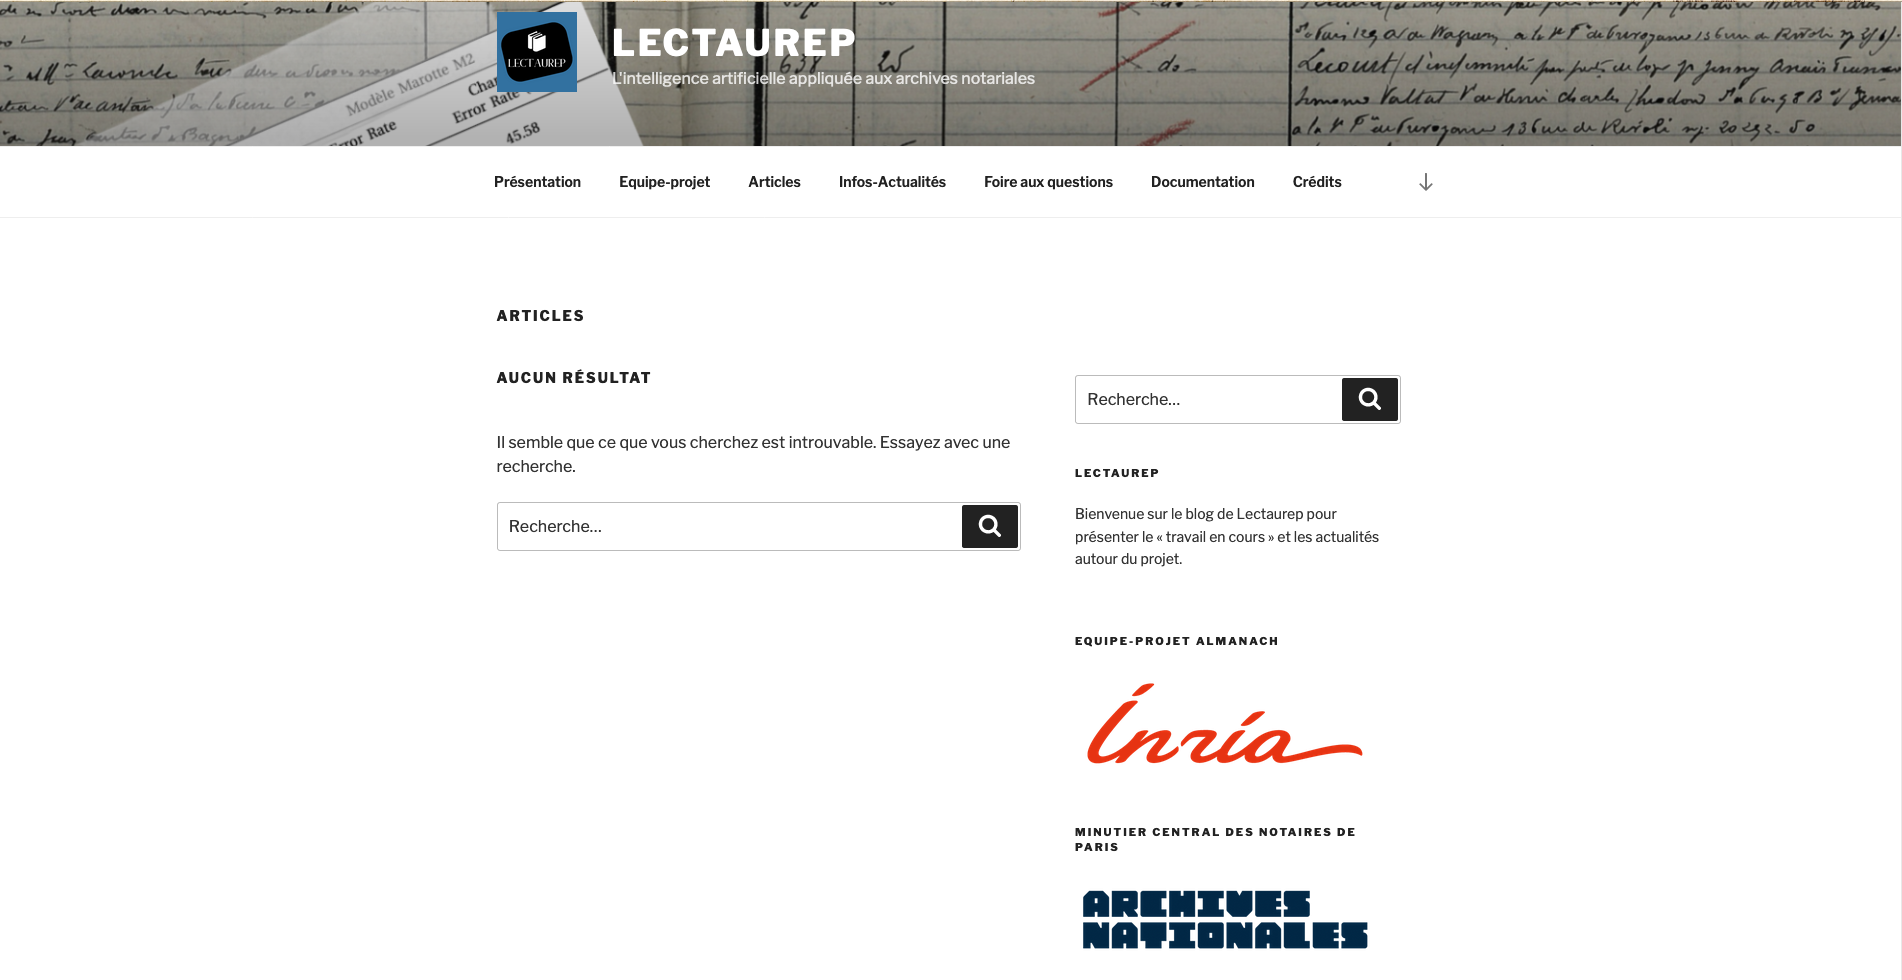
\includegraphics[width=18cm]{images_annexes/blog_lectaurep.png}}}
    \caption{Blog hypotheses.org Lectaurep \textcopyright L. Terriel, blog hypotheses.org Lectaurep}
    \label{fig:blog_lectaurep}
\end{figure}


\chapter{Format pivot XML TEI Lectaurep}
localisation : \citecode{/B-Format\_pivot\_XML\_TEI\_Lectaurep} contenant :
\skip
\dirtree{%
.1 /B-Format\_pivot\_XML\_TEI\_Lectaurep/.
   .2 Doc/\DTcomment{regroupe la documentation sur le projet de format pivot XML TEI pour Lectaurep}.
        .3 Modélisation\_et\_documentation\_format\_pivot/.
           .4 template\_pivot\_TEI\_lectaurep.xml\DTcomment{Canevas pour formaliser les attentes et les réflexions des acteurs pour l'inclusion des données Lectaurep dans la TEI.}.
           .4 Les ODD aux formats : XML, PDF et HTML.\DTcomment{La documentation standard TEI pour le format pivot TEI Lectaurep.}.
           .4 oddbyexample.xsl\DTcomment{Une feuille de transformation XSL pour générer une nouvelle ODD à partir de la template pivot.}.
        .3 Crosswalks\_vers\_TEI\DTcomment{Un ensemble de transformations XSL utiles vers les spécifications TEI et ALTO, issues de différents projets.}.
            .4 ALTO -> TEI.
            .4 EAD -> TEI (2 versions).
            .4 ALTO -> TEI.
            .4 PAGE -> ALTO.
   .2 Generator\_Lectaurep2TEI/\DTcomment{CLI Python permettant de simuler 
	                                     la conversion des données issues de Lectaurep (EAD-EAC, ALTO, EXIF) 
	                                     vers un format XML TEI Pivot suivant les recommandations de l'ODD 
	                                     (voir le readme.md pour plus de détails).}.
        .3 Output/\DTcomment{Dossier dans lequel est généré la sortie du script.}.
            .4  test\_legay\_tei.xml\DTcomment{Format pivot TEI Lectaurep de test généré en sortie du script.}.
        .3 Sets\_test\_Legay/\DTcomment{Contient un ensemble de fichiers correspondant aux données fournies par Lectaurep pour tester le script Lectaurep2TEI et généré une première version du format pivot.}.
            .4  Data\_xml\_alto/\DTcomment{fichiers XML ALTO correspondants aux transcriptions vérité terrain récupérés sur ShareDocs relatives aux images numérisées du répertoire de notaire d'Ernest Legay (étude XXIII).}.
            .4  Data\_xml\_ead\_eac/\DTcomment{fichiers XML EAD et XML EAC-CPF correpondants aux instruments de recherche des répertoires du notaire Ernest Legay (étude XXIII) et notices producteurs récupérés sur la Salle des inventaires virtuels des Archives nationales.}.
                .5 FRAN\_IR\_041698.xml \DTcomment{IR \inquote{Minutes et répertoires du notaire Ernest LEGAY, 25 février 1875 - 14 mai 1902 (étude XXIII)}.}.
                .5 FRAN\_IR\_051379.xml \DTcomment{IR \inquote{Images des répertoires du notaire Ernest Legay pour l'étude XXIII}.}.
                .5 FRAN\_NP\_010150.xml \DTcomment{Notice producteur de l'étude XXIII.}.
                .5 FRAN\_NP\_010150.xml \DTcomment{Notice producteur de Legay, Ernest.}.
                .5 Schémas XML et DTD EAD et EAC-CPF.
            .4  images/\DTcomment{Images numérisées du répertoire de notaire d'Ernest Legay (étude XXIII) issues du Golden Set de ShareDocs.}.
        .3 generator\_utils/.\DTcomment{Ensemble des modules Python utiles au fonctionnement du CLI generator Lectaurep2TEI. Pour les usages consulter les \textit{docstrings}.}.
            .4  \_\_init\_\_.py.
            .4  build\_utils.py.
            .4  extract\_utils.py.
            .4  validation\_utils.py.
        .3 pack\_schemaRNG/.\DTcomment{Doit accueillir à terme les schémas de validation Relax NG du format pivot XML TEI Lectaurep.}.
            .4 tei\_all.rng.\DTcomment{Schéma Relax NG TEI ALL.}.
        .3 Lectaurep\_ALTO2TEI.xsl.\DTcomment{Une feuille de transformation XSL ALTO vers TEI nécéssaire pour le fonctionnement du script principal. Pour les usages consulter la \textit{docstring}.}.
        .3 Lectaurep\_EADEAC2TEI.xsl.\DTcomment{Une feuille de transformation XSL EAD/EAC vers TEI nécéssaire pour le fonctionnement du script principal. Pour les usages consulter la \textit{docstring}.}.
        .3 catalog\_alto.xml.\DTcomment{Fichier automatiquement créé par le script, nécéssaire pou l'usage de la fonction Xpath 2.0 \citecode{collection()} pour la feuille XSL \citecode{Lectaurep\_ALTO2TEI.xsl}}.
        .3 catalog\_ead\_eac.xml.Lectaurep\_ALTO2TEI.xsl\DTcomment{Fichier automatiquement créé par le script, nécéssaire pou l'usage de la fonction Xpath 2.0 \citecode{collection()} pour la feuille XSL \citecode{Lectaurep\_EADEAC2TEI.xsl}}.
        .3 generator\_Lectaurep2TEI\_logo.png.
        .3 inr\_logo\_grisbleu.png.
        .3 main.py.\DTcomment{Script Python principal d'exécution du CLI generator Leactaurep2TEI.}.
        .3 readme.md.\DTcomment{Documentation pour installer et lancer le programme.}.
        .3 requirements.txt.\DTcomment{Ensemble des \textit{packages} Python nécessaires à l'utilisation du CLI}.
        .3 snap\_generator.png.
        }

\chapter{Application Kraken Benchmark}
localisation : \citecode{/C-Application\_Kraken\_Benchmark} contenant :
\skip
\dirtree{%
.1 /C-Application\_Kraken\_Benchmark/.
   .2 Documentation-Reasearch/.\DTcomment{Contient les versions du \textit{notebook Jupyter} exposant les réflexions sur les métriques et les algorithmes utilisés dans l'application Kraken-Benchmark.}.
    .3 Evaluation de la similarité entre deux séquences dans le contexte de la reconnaisance automatique de caractères.\DTcomment{\textit{notebook Jupyter} en versions PDF, HTML et IPYNB (format natif).}. 
    .3 Ensemble d'images rattachés au \textit{notebook Jupyter}.
   .2 KB-app/.\DTcomment{Dossier contenant les fichiers pour faire fonctionner l'application Kraken-Benchmark.}.
    .3 STS\_Tools/.\DTcomment{Le \textit{package} Python \textit{Sequences to Similarity} créée pour l'application Kraken-Benchmark contient deux modules Python.}.
        .4 STSig.py.\DTcomment{module Python \textit{Sequences To Signals} (en cours de développement); expérience pour visualiser et comparer deux chaînes de caractères sous la forme de signaux.}.
        .4 SynSemTS.py.\DTcomment{module Python \textit{Syntactic Semantic To Similarity} qui contient la plupart des métriques (syntaxiques et sémantiques) utilisé dans l'application pour l'analyse deux chaînes de caractères correspondant à la vérité terrain et la transcription issue du système HTR.}.
        .4  \_\_init\_\_.py.
    .3 kb\_report/.\DTcomment{Dossier contenant les fichiers pour la gestion de la partie affichage dans le navigateur de l'application en \textit{Flask}.}.
        .4  static/.\DTcomment{contient les images de l'application à afficher dans le navigateur.}.
        .4  templates/.\DTcomment{contient les pages HTML de l'application.}.
        .4  \_\_init\_\_.py.
        .4  routing.py\DTcomment{Script Python qui contient les différentes routes URL de l'application.}.
    .3 kb\_utils/.\DTcomment{Dossier contenant un module Python nécessaire au fonctionnement de l'application.}.
        .4  \_\_init\_\_.py.
        .4  kb\_utils.py.\DTcomment{Module Python contenant des fonctions utiles au fonctionnement de l'application.}.
    .3 environment.yml.\DTcomment{Fichier pour la création d'un environnement virtuel \textit{Conda} contenant les \textit{packages} Python nécéssaires.}.
    .3 kraken\_benchmark.py.\DTcomment{Script principal pour l'exécution de l'application Kraken-Benchmark.}.
   .2 sets\_test/.\DTcomment{Jeux de fichiers pour effectuer des tests dans Kraken-Benchmark et scripts Python.}.
    .3 jules\_verne\_set\_test/.\DTcomment{Jeux de données utilisés pour tester l'application au fur et à mesure des développements.}.
        .4  images/.\DTcomment{Contient des numérisations (formats \citecode{.jpeg}) de l'ouvrage \textit{Voyage au centre de la terre} récupérés sur Gallica.}.
        .4  dataset\_GT/.\DTcomment{Contient les transcriptions vérités terrains en format texte brut utilisées pour comparer les résultats issus de l'HTR de Kraken-Benchmark. Édités à partir du CLI Kraken.}.
        .4  model/.\DTcomment{Contient le modèle (format \citecode{.mlmodel}) entraîné sur le CLI Kraken pour réaliser l'OCR dans Kraken-Benchmark sur le set de numérisations de \textit{Voyage au centre de la terre}.}.
    .3 sets\_tests\_lectaurep/.\DTcomment{Jeux de données utilisés pour tester les modèles de transcription issus du CLI Kraken sur des images de répertoires de notaires sélectionnés pour leurs particularismes (pour plus de détails sur les sets d'images et les modèles HTR utilisés voir le fichier \citecode{CR\_tests\_lectaurep\_KB.md}) pour évaluer la qualité des transcriptions durant le stage.}.
        .4  different\_control\_set/.\DTcomment{Contient les transcriptions vérité terrains (\citecode{GT} et les images).}.
        .4  homogeneous\_control\_set/.\DTcomment{Contient les transcriptions vérité terrains (\citecode{GT} et les images).}.
        .4  set\_material\_defects/.\DTcomment{Contient les transcriptions vérité terrains (\citecode{GT} et les images).}.
        .4  set\_writing\_defects/.\DTcomment{Contient les transcriptions vérité terrains (\citecode{GT} et les images).}.
        .4  snaps\_tests\_lectaurep/.\DTcomment{Contient des captures sous la forme de fichier HTML de l'application Kraken-Benchmark réalisés lors des différents tests.}.
            .5 report\_html/.\DTcomment{Contient des captures de la page d'accueil de Kraken-Benchmark avec les principales métriques.}.
            .5 versus\_text\_html/.\DTcomment{Contient des captures de la fonctionnalité de comparaison de la vérité terrain et de la transcription HTR dans Kraken-Benchmark.}.
        .4  models/.\DTcomment{Contient les modèles HTR, entraînés avec le CLI Kraken, et utilisés sur les différents jeux de données.}.
        .4  CR\_tests\_lectaurep\_KB.md\DTcomment{Compte-rendu présentant le déroulement des tests, la description des sets de tests, des modèles et des résultats des expériences.}.
        .4  details\_data\_average\_tests\_model\_test\_lectaurep\_bin\_accuracy\_6064.mlmodel - Feuille 1.pdf\DTcomment{Fichier PDF présentant la moyenne des résultats des tests avec le modèle 6064, utilisé pour le graphique radar.}.
        .4   details\_data\_average\_tests\_model\_test\_lectaurep\_bin\_accuracy\_8164.mlmodel - Feuille 1.pdf\DTcomment{Fichier PDF présentant la moyenne des résultats des tests avec le modèle 8164, utilisé pour le graphique radar.}.
        .4   radar\_test\_II\_model\_0-8164.png.
        .4  radar\_test\_I\_model\_0-6064.png.
    .3 alto2text.py.\DTcomment{Script Python adapté, provenant de la \textit{StaatsbibliothekBerlin} permettant la conversion de certaines transcriptions vérités terrains en XML ALTO vers des fichiers texte brut.}.
    .3 radar\_graph.py.\DTcomment{Script Python adapté permettant la génération d'un graphique radar, utile pour le rapport concernant les tests spécifiques à Lectaurep durant le stage.}.
   .2 README.md.\DTcomment{Présentation et documentation pricipale de l'application pour l'installation et l'utilisation.}.
   }

\chapter{Scripts Python complémentaires}
\begin{figure}[h]
\lstset{language=Python}
\begin{lstlisting}
"""
Exemple de script pour l'étiquetage morpho-syntaxique (POS)

Auteur : Lucas Terriel
Date : 14/09/2020
"""

# On importe le package spacy (pour le NLP)
import spacy
from spacy import displacy

# On charge un modèle français
# ! préalable télécharger le modèle (réseau convolutionnel entraîné sur deux corpus, WikiNER et Sequoia) !
# python -m spacy download fr_core_news_sm
model_fr = spacy.load("fr_core_news_sm")

# On défini une phrase de test
test = "Dussuel (par Paul Charles Claude) demeurant à Paris"

def return_POS(sentence):
    """
    fonction pour tokeniser la phrase et retourner les étiquettes grammaticale
    de chaque token.

    :param sentence: phrase
    :type sentence: str
    :return: token et étiquettes POS
    :type return : list
    """
    # Tokenise la phrase
    document = model_fr(sentence)
    # Retourne les étiquettes de chaque token dans une liste en compréhension
    return [{(X, X.pos_)} for X in document]

# affichage de la liste
print(return_POS(test))

# Pour la visualisation POS on défini les options
options = {"color": "red", "font": "Source Sans Pro"}

# Visualisation POS
doc = model_fr(test)
displacy.serve(doc, style="dep", options=options)

\end{lstlisting}
\caption{Script Python pour effectuer de l'étiquetage morpho-syntaxique (POS) \textcopyright L. Terriel, 2020}
\label{fig:script_python_POS}
\end{figure}